\documentclass[{../RL_for_QSP.tex}]{subfiles}

\begin{document}
    \section{Background Information}
    \label{sec:BI}

\subsection{Quantum States}   
To discuss quantum state preparation, it is first necessary to define quantum states. In quantum computers, the fundamental unit of information is the quantum bit or qubit. Unlike classical computers, which work in a binary system of $0$s and $1$s, qubits can exist in a state of superposition. When a property of a qubit, such as spin or momentum, is measured, the state of superposition collapses into one of two possible outcomes. Often these outcomes are labelled as $0$ or $1$, although the use of $1$ and $-1$ is also common. 
%Two states are distinguishable if there is a precise experiment that can tell them apart. In mathematical terms, two states are distinguishable if they are orthogonal.

Quantum mechanical states are defined in Hilbert spaces. The most convenient way to represent a qubit is in $\mathbb{C}^2$ with orthonormal basis vectors:
\begin{equation*}
    \ket{0} = \begin{pmatrix}1\\ 0\end{pmatrix} \text{ and }\\
    \ket{1} = \begin{pmatrix}0\\ 1\end{pmatrix}.
\end{equation*}
The superposition state $\ket{\psi}$ of a qubit can be represented as $\ket{\psi} = a_0\ket{0} + a_1\ket{1}$. Here $a_0$ and $a_1$ are the complex scalar amplitudes of measuring $0$ and $1$ respectively. Amplitudes are like probabilities but must be complex to account for quantum effects (superposition and entanglement). $\ket{\psi}$ is a unit vector.

\begin{equation*}
\begin{aligned}
1 &= \braket{\psi} \\
&= (\bar{a_0}\bra{0} + \bar{a_1}\bra{1}) \cdot (a_0\ket{0} + a_1\ket{1}) \\
&= |a_0|^2\braket{0} + |a_1|^2\braket{1} + \bar{a_0}a_1\braket{0}{1} + \bar{a_1}a_0\braket{1}{0} \\
&= |a_0|^2 + |a_1|^2
\end{aligned}
\end{equation*}

The squares of the absolute values of amplitudes in a quantum system must add to 1. The probability of observing a single state from the superposition is obtained by squaring the absolute value of its amplitude. The state of a qubit $\ket{\psi} = a_0\ket{0} + a_1\ket{1}$ can also be represented by points $(\theta, \phi)$ on the unit sphere (also called Bloch sphere) depicted in Figure \ref{Bloch sphere}. Here, 
$$\ket{\psi} = \cos(\frac{\theta}{2})\ket{0} + e^{i\phi}\sin(\frac{\theta}{2})\ket{1}.$$ 

\begin{figure}[H]
	\centering
	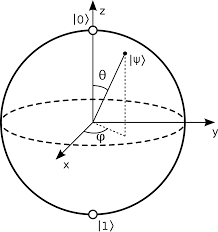
\includegraphics[scale=0.75]{Bloch Sphere.png}
	\caption{Bloch sphere}
	\label{Bloch sphere}
\end{figure}

\subsection{Quantum State Evolution}

The basic dynamical assumption of quantum mechanics is that knowing the state at one time, the quantum equations of motion determine what it will be later. The state at time $t$, denoted $\ket{\psi(t)}$, is given by some operation $U(t)$ acting on the state at time $0$. That is, $\ket{\psi(t)} = U(t)\ket{\psi(0)}$. Time evolution in quantum mechanics is linear and unitary. Note that the time evolution of the state-vector is deterministic. Just as in classical physics, incremental change in time leads to a differential equation for the evolution of the state vector:
\begin{equation} \label{shr}
    i \hslash \frac{\partial \ket{\psi}}{\partial t} = H \ket{\psi}.
\end{equation}

Eqn. \ref{shr} is called the generalized Shrödinger equation or the time-dependent Schrödinger equation. $\hslash \approx 1.05457 \times 10^{-34} \: kg \: m^2/s$ is the reduced Planck constant, from now on taken to be $1$ for simplicity. $H$ is called the quantum Hamiltonian. It can be represented as a Hermitian matrix and its eigenvalues are the values that would result from measuring the energy of a quantum system. The Hamiltonian differs between quantum systems and is often derived through experimentation. Given an initial state $\ket{\psi_i}$, the solution to Eqn. \ref{shr} is easily derived and presented in Eqn. \ref{shrsol}.

\begin{equation}\label{shrsol}
    \ket{\psi(t)} = e^{-iH t}\ket{\psi_i}
\end{equation}

\subsection{Spin in a Magnetic Field}
Quantum spin is a property, just like position and momentum, that can be attributed to particles (electrons, quarks, neutrinos etc.). The quantum spin is a quantum system in its own right. Just as the Hamiltonian is an operator related to the energy of a system, there are spin operators. Again, these operators are Hermitian matrices whose eigenvalues correspond to the two possible outcomes of measuring the spin component in a specific direction. By convention, the basis states $\ket{0}$ and $\ket{1}$ are taken to be spin up and spin down on the $z$-axis. The possible outcomes of measurement along the $z$-axis are spin $+1$ and spin $-1$. Similarly, the spin can be measured along the $x$-axis and $y$-axis. In this case, the orthogonal states are $\frac{1}{\sqrt{2}}\ket{0} + \frac{1}{\sqrt{2}}\ket{1}$ and $\frac{1}{\sqrt{2}}\ket{0} - \frac{1}{\sqrt{2}}\ket{1}$, and $\frac{1}{\sqrt{2}}\ket{0} + \frac{i}{\sqrt{2}}\ket{1}$ and $\frac{1}{\sqrt{2}}\ket{0} - \frac{i}{\sqrt{2}}\ket{1}$ respectively. Altogether, this yields the following spin operators:

\begin{align*}
    &\sigma_z = \begin{pmatrix}
    1 & 0 \\
    0 & -1
    \end{pmatrix} \\
    &\sigma_x = \begin{pmatrix}
    0 & 1 \\
    1 & 0
    \end{pmatrix} \\
    &\sigma_y = \begin{pmatrix}
    0 & -i \\
    i & 0
    \end{pmatrix}.
\end{align*}

Particles can have a permanent magnetic moment along the direction of their spin, and this magnetic moment gives rise to electromagnetic interactions that depend on the spin. An example Hamiltonian for a two-level spin system controlled by magnetic fields $h_t^x$ and $h_t^z$ applied along the $x$-axis and $z$-axis is given in Eqn. \ref{spinhaml}.

\begin{equation}\label{spinhaml}
    H = -h^x_t\sigma_x - h^z_t\sigma_z
\end{equation}

The Hamiltonian specified in Eqn. \ref{spinhaml} and the differential equation in Eqn. \ref{shr} together with some initial state $\ket{\psi_i}$ and desired state $\ket{\psi_f}$ provide a control problem. 

\subsection{Noise}
% https://arxiv.org/pdf/2006.16421.pdf - Gaussian distributed
%Quantum Noise and Error Correction. (n.d.). Quantum Computing Explained, 251–278. doi:10.1002/9780470181386.ch12  - Dephasing 
%https://www.youtube.com/watch?v=Dj7HNmP230o https://arxiv.org/pdf/2012.08827.pdf - D-Wave

Perhaps the greatest challenge in quantum computing arises from errors broadly known as decoherence. Dephasing is a common source of error which occurs when there is fluctuation in a magnetic field along the $z$-axis \cite{w2007quantum}. When some dephasing noise $\eta_t$ is introduced to the Hamiltonian in Eqn. \ref{spinhaml}, it becomes a stochastic control problem which can be solved using reinforcement learning. The system is now that shown in Eqn. \ref{noisectrl}.
\begin{equation}\label{noisectrl}
     i \hslash \frac{\partial \ket{\psi}}{\partial t} = (\eta_t \sigma_z -h^x_t \sigma_x - h^z_t\sigma_z) \ket{\psi}
\end{equation}
The noise $\eta_t$ can be modelled as a Gaussian distribution with zero mean \cite{Zaborniak2021}. 
% When such noise was benchmarked in D-Wave Quantum Annealers, the variance was found to be around $\sigma^2 = 0.05$.

% The underlying reason for q-learning can be traced back to the non-integrability of the dynamical many-body system, as a result of which the solution of the Schrödinger equation cannot be written down as a closed-form expression even for a fixed protocol, and the situation is much more complicated when one starts optimizing over a family of protocols


\end{document}